% This is a template for doing homework assignments in LaTeX

\documentclass{article} % This command is used to set the type of document you are working on such as an article, book, or presenation

\usepackage{geometry} % This package allows the editing of the page layout
\usepackage{amsmath}  % This package allows the use of a large range of mathematical formula, commands, and symbols
\usepackage{graphicx}  % This package allows the importing of images
\usepackage{amssymb}

\newcommand{\question}[2][]{\begin{flushleft}
        \textbf{Question #1}: \textit{#2}

\end{flushleft}}
\newcommand{\sol}{\textbf{Solution}:} %Use if you want a boldface solution line
\newcommand{\maketitletwo}[2][]{\begin{center}
        \Large{\textbf{Assignment #1}
            
            EEE554} % Name of course here
        \vspace{5pt}
        
        \normalsize{Yan Xiao Chen  % Your name here
        
        \today}        % Change to due date if preferred
        \vspace{15pt}
        
\end{center}}
\begin{document}
    \maketitletwo[4]  % Optional argument is assignment number
    %Keep a blank space between maketitletwo and \question[1]

    \question[1]{Problem 1} 
    1a. A is 1, see earlier pages for work \\
    1b. $Z = V/U$, $S_Z=0 < z < \frac{1}{2}$, see earlier pages for work

    Intersection point of curve is $(\frac{1}{1-z},\frac{1}{1-z}-1)$
    
    $F_Z(z)=Pr(V \leq uz)= 1 - Pr(V \geq uz)$

    $Pr(V \geq uz)=1-\int_{u=\frac{1}{1-z}}^{2} \int_{v=uz}^{u-1}u+v \quad dv du$, $\forall \ 0<z<\frac{1}{2}$

    $Pr(V \geq uz)=\int_{u=\frac{1}{1-z}}^{2}(u^2-u-u^2z+\frac{1}{2}u^2-u+\frac{1}{2}-\frac{u^2z^2}{2})du$, $\forall \ 0<z<\frac{1}{2}$

    $Pr(V \geq uz)=\int_{u=\frac{1}{1-z}}^{2}((1-z+\frac{1}{2}-\frac{1}{2}z^2)u^2+-2u^2+\frac{1}{2})du$, $\forall \ 0<z<\frac{1}{2}$

    $Pr(V \geq uz)=(\frac{3}{2}-z-\frac{1}{2}z^2)(\frac{1}{3})(2^3-(\frac{1}{1-z})^3)-(4-(\frac{1}{1-z})^2)+\frac{1}{2}(2-\frac{1}{1-z})$, $\forall \ 0<z<\frac{1}{2}$
    
    $\Rightarrow F_Z(z)=1-(\frac{3}{2}-z-\frac{1}{2}z^2)(\frac{1}{3})(2^3-(\frac{1}{1-z})^3)-(4-(\frac{1}{1-z})^2)+\frac{1}{2}(2-\frac{1}{1-z})$, $\forall \ 0<z<\frac{1}{2}$

    $\therefore F_Z(z) = \left\{ \begin{array}{cl}
        0  &  \ x < 0 \\
        1-(\frac{3}{2}-z-\frac{1}{2}z^2)(\frac{1}{3})(2^3-(\frac{1}{1-z})^3)-(4-(\frac{1}{1-z})^2)+\frac{1}{2}(2-\frac{1}{1-z}) &  \ 0 \leq x < \frac{1}{2} \\
        1  &  otherwise 
        \end{array} \right.$
    
    \begin{figure}[h!]
        \centering
        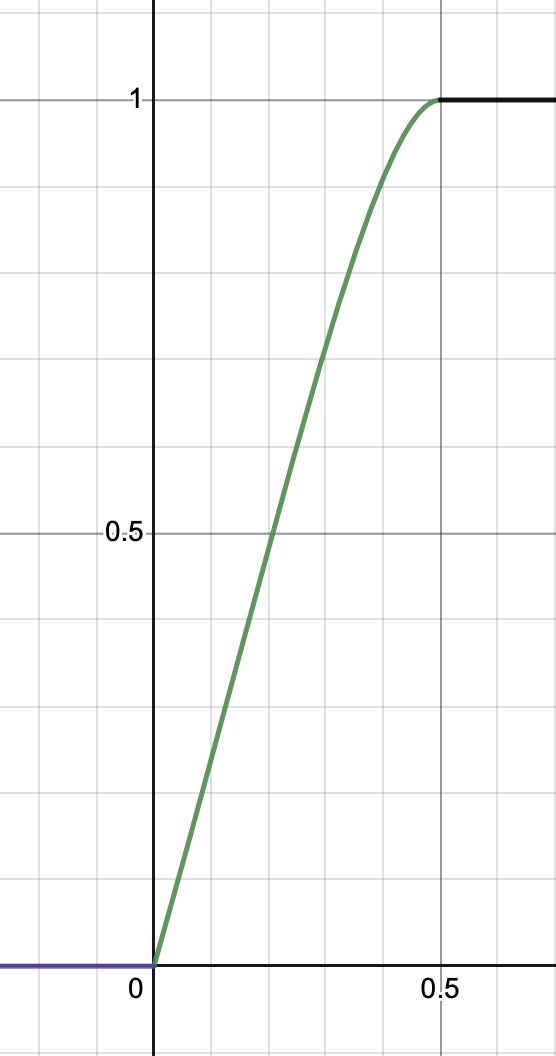
\includegraphics[scale=0.20]{HW/HW4/p1b.jpg}
        \label{fig:$F_Z$}
        \caption{$F_Z$}    
    \end{figure}
    
    \newpage

    1c. $W=U+V$, $S_W=1 < w < 3$, see earlier pages for work

    Intersection point of curve is $(\frac{w+1}{2},\frac{w+1}{2}-1)$

    $F_W(w)=Pr(V \leq w-u)$

    \begin{figure}[h]
        \centering
        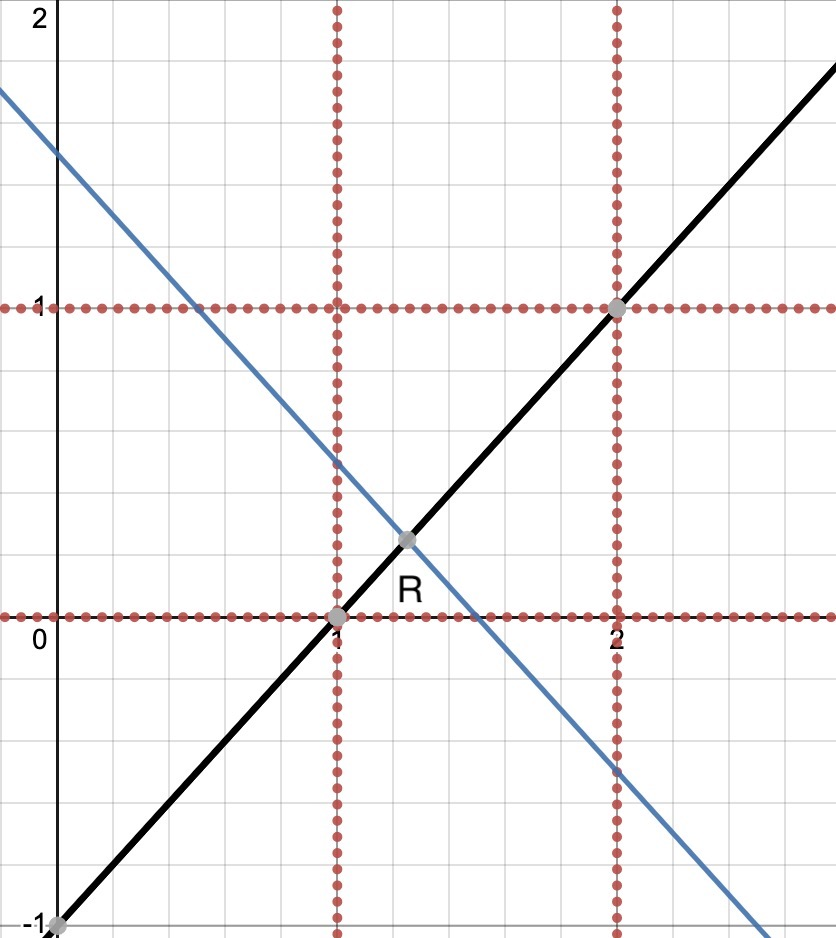
\includegraphics[scale=0.25]{HW/HW4/p1c_case1.jpg}
        \label{fig:$F_W$}
        \caption{Case 1, blue is the $v = w-u$, black is $v = u-1$, region R is the region of interest}    
    \end{figure}
    
    Case 1: if $1 \leq \frac{w+1}{2} < 2$

    $F_W(w)=\int_{u=1}^{\frac{w+1}{2}}\int_{v=0}^{u-1}u+v \ dvdu + \int_{u=\frac{w+1}{2}}^{w}\int_{v=0}^{w-u}u+v \ dvdu$, $\forall \ 1 < w <2$

    $F_W(w)=\int_{u=1}^{\frac{w+1}{2}}\frac{3}{2}u^2-2u+\frac{1}{2}\ du+\int_{u=\frac{w+1}{2}}^{w}-\frac{1}{2}u^2+\frac{1}{2}w^2\ du$, $\forall \ 1 < w <2$

    $F_W(w)=\frac{1}{2}((\frac{w+1}{2})^3-1)-((\frac{w+1}{2})^2-1)+\frac{1}{2}(\frac{w+1}{2}-1))-\frac{1}{6}(w^3-(\frac{w+1}{2})^3)+\frac{1}{2}w^2(w-\frac{w+1}{2})$, $\forall 1 < w <2$
\newpage
\begin{figure}[]
    \centering
    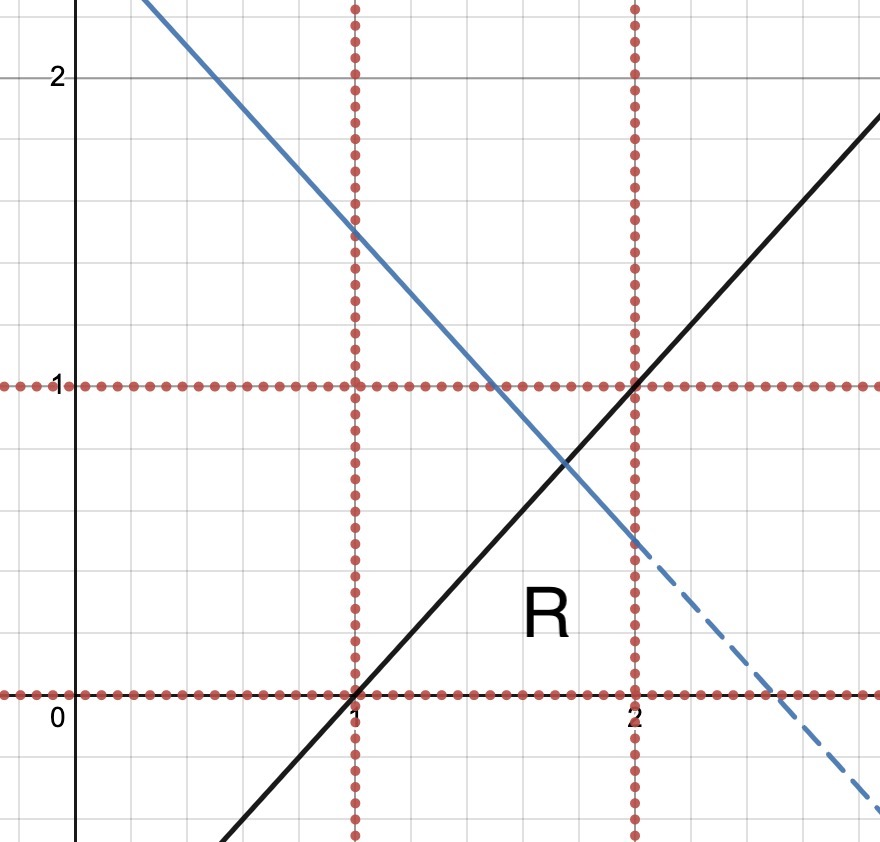
\includegraphics[scale=0.20]{HW/HW4/p1c_case2.jpg}
    \label{fig:$F_W,2$}
    \caption{Case 2, blue is the $v = w-u$, black is $v = u-1$, region R is the region of interest}    
\end{figure}

    Case 2: if $2 \leq \frac{w+1}{2} < 3$

    $F_W(w)=\int_{u=1}^{\frac{w+1}{2}}\int_{v=0}^{u-1}u+v \ dvdu + \int_{\frac{w+1}{2}}^{2}\int_{v=0}^{w-u}u+v \ dvdu$, $\forall \ 2<w<3$

    $F_W(w)=\int_{u=1}^{\frac{w+1}{2}}\frac{3}{2}u^2-2u+\frac{1}{2} \ du + \int_{\frac{w+1}{2}}^{2}-\frac{1}{2}u^2+\frac{1}{2}w^2 \ du$, $\forall \ 2<w<3$

    $F_W(w)=\frac{1}{2}((\frac{w+1}{2})^3-1)-((\frac{w+1}{2})^2-1)+\frac{1}{2}(\frac{w+1}{2}-1)-\frac{1}{6}(2^3-(\frac{w+1}{2})^3)+\frac{1}{2}w^2(2-\frac{w+1}{2})$, $\forall \ 2<w<3$ \\

    \begin{figure}[]
        \centering
        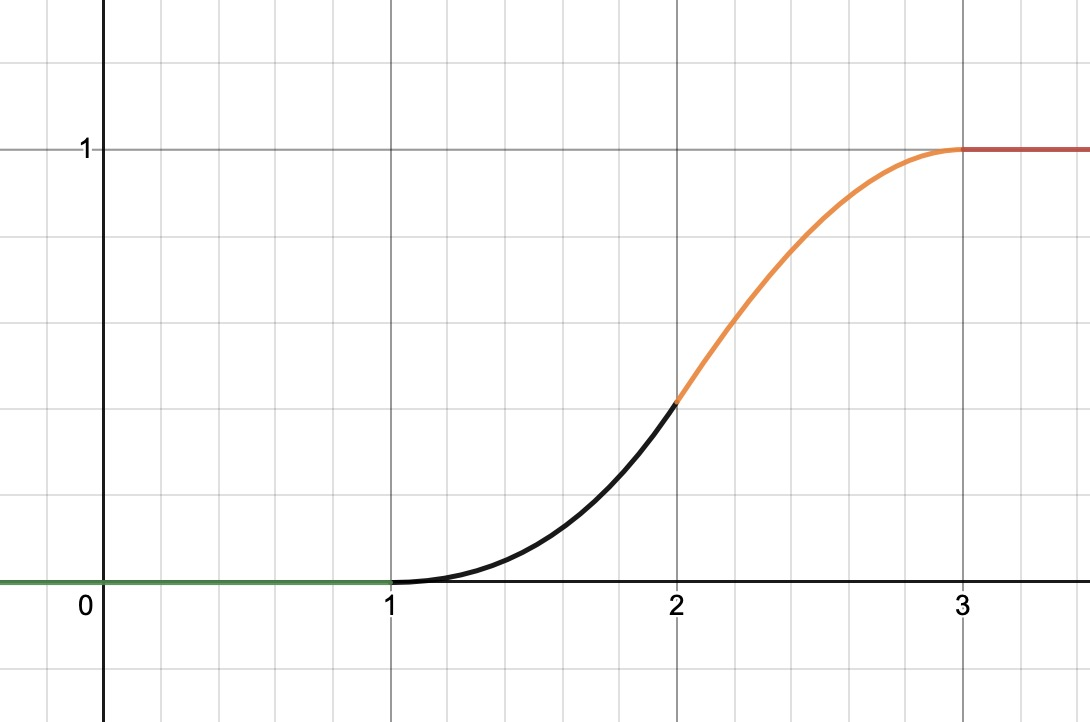
\includegraphics[scale=0.20]{HW/HW4/p1c_fw.jpg}
        \label{fig:$F_W,all$}
        \caption{$F_W$ for all w}    
    \end{figure}

    $\therefore$ Let $k=\frac{w+1}{2}$
    
    $F_Z(z) = \left\{ \begin{array}{cl}
        0  &  \ w < 1 \\
        \frac{1}{2}(k^3-1)-(k^2-1)+\frac{1}{2}(k-1)+-\frac{1}{6}(w^3-k^3)+\frac{1}{2}w^2(w-k) &  \ 1 \leq w < 2 \\
        \frac{1}{2}(k^3-1)-(k^2-1)+\frac{1}{2}(k-1)+-\frac{1}{6}(2^3-w^3)+\frac{1}{2}w^2(2-k)  &  \ 2 \leq w < 3 \\
        1 &  \ w \geq 3 \\
        \end{array} \right.$
\newpage
    1d.

    $$Z = \frac{V}{U}$$
    $$W = V+U$$
    $$\Rightarrow U(w,z)=\frac{W}{1+Z}, \text{ and } V(z,w)=\frac{ZW}{1+Z}$$

    $$\because S_{uv}=\{{\{u| 1 \leq u < 2\},\{v| 0 \leq v < 1\},\{(u,v)| v \leq u-1 \}}\}$$

    $$\therefore S_{wz}=\{{\{u(w,z)| 1 \leq \frac{w}{1+z} < 2\},\{v(w,z)| 0 \leq \frac{zw}{1+z} < 1\},\{(u,v)| \frac{zw}{1+z} \leq \frac{w}{1+z}-1 \}}\}$$
    \question[2]{Problem 2}
    
    2a-2b please see attachment.

    2c. Picture please see attachment below. When M is small, the transformation using histogram do not match the expected probability density function. As M grows by couple decades, the probability density function using histogram match the expected probability density function.  
    
%    \question[3]{What is the \Large{$\int_0^2 x^2 \, dx $}\normalsize{. Show all steps}}
    
%    \begin{align*}
%    \int_0^2 x^2 &= \left. \frac{x^3}{3} \right|_0^2 \\
%                 &= \frac{2^3}{3}-\frac{0^3}{3}\\
%                 &= \frac{8}{3}
%    \end{align*}
\end{document}